% Options for packages loaded elsewhere
% Options for packages loaded elsewhere
\PassOptionsToPackage{unicode}{hyperref}
\PassOptionsToPackage{hyphens}{url}
\PassOptionsToPackage{dvipsnames,svgnames,x11names}{xcolor}
%
\documentclass[
]{rapportCS}
\usepackage{xcolor}
\usepackage{amsmath,amssymb}
\setcounter{secnumdepth}{5}
\usepackage{iftex}
\ifPDFTeX
  \usepackage[T1]{fontenc}
  \usepackage[utf8]{inputenc}
  \usepackage{textcomp} % provide euro and other symbols
\else % if luatex or xetex
  \usepackage{unicode-math} % this also loads fontspec
  \defaultfontfeatures{Scale=MatchLowercase}
  \defaultfontfeatures[\rmfamily]{Ligatures=TeX,Scale=1}
\fi
\usepackage{lmodern}
\ifPDFTeX\else
  % xetex/luatex font selection
\fi
% Use upquote if available, for straight quotes in verbatim environments
\IfFileExists{upquote.sty}{\usepackage{upquote}}{}
\IfFileExists{microtype.sty}{% use microtype if available
  \usepackage[]{microtype}
  \UseMicrotypeSet[protrusion]{basicmath} % disable protrusion for tt fonts
}{}
\makeatletter
\@ifundefined{KOMAClassName}{% if non-KOMA class
  \IfFileExists{parskip.sty}{%
    \usepackage{parskip}
  }{% else
    \setlength{\parindent}{0pt}
    \setlength{\parskip}{6pt plus 2pt minus 1pt}}
}{% if KOMA class
  \KOMAoptions{parskip=half}}
\makeatother
% Make \paragraph and \subparagraph free-standing
\makeatletter
\ifx\paragraph\undefined\else
  \let\oldparagraph\paragraph
  \renewcommand{\paragraph}{
    \@ifstar
      \xxxParagraphStar
      \xxxParagraphNoStar
  }
  \newcommand{\xxxParagraphStar}[1]{\oldparagraph*{#1}\mbox{}}
  \newcommand{\xxxParagraphNoStar}[1]{\oldparagraph{#1}\mbox{}}
\fi
\ifx\subparagraph\undefined\else
  \let\oldsubparagraph\subparagraph
  \renewcommand{\subparagraph}{
    \@ifstar
      \xxxSubParagraphStar
      \xxxSubParagraphNoStar
  }
  \newcommand{\xxxSubParagraphStar}[1]{\oldsubparagraph*{#1}\mbox{}}
  \newcommand{\xxxSubParagraphNoStar}[1]{\oldsubparagraph{#1}\mbox{}}
\fi
\makeatother


\usepackage{longtable,booktabs,array}
\newcounter{none} % for unnumbered tables
\usepackage{calc} % for calculating minipage widths
% Correct order of tables after \paragraph or \subparagraph
\usepackage{etoolbox}
\makeatletter
\patchcmd\longtable{\par}{\if@noskipsec\mbox{}\fi\par}{}{}
\makeatother
% Allow footnotes in longtable head/foot
\IfFileExists{footnotehyper.sty}{\usepackage{footnotehyper}}{\usepackage{footnote}}
\makesavenoteenv{longtable}
\usepackage{graphicx}
\makeatletter
\newsavebox\pandoc@box
\newcommand*\pandocbounded[1]{% scales image to fit in text height/width
  \sbox\pandoc@box{#1}%
  \Gscale@div\@tempa{\textheight}{\dimexpr\ht\pandoc@box+\dp\pandoc@box\relax}%
  \Gscale@div\@tempb{\linewidth}{\wd\pandoc@box}%
  \ifdim\@tempb\p@<\@tempa\p@\let\@tempa\@tempb\fi% select the smaller of both
  \ifdim\@tempa\p@<\p@\scalebox{\@tempa}{\usebox\pandoc@box}%
  \else\usebox{\pandoc@box}%
  \fi%
}
% Set default figure placement to htbp
\def\fps@figure{htbp}
\makeatother





\setlength{\emergencystretch}{3em} % prevent overfull lines

\providecommand{\tightlist}{%
  \setlength{\itemsep}{0pt}\setlength{\parskip}{0pt}}



 


% Neutralise le \maketitle par défaut de Pandoc : la page de garde est
% entièrement gérée par \fairecouverture (gabarit ENSAI) plus bas.
\renewcommand{\maketitle}{}

%----------- Informations du rapport ---------
\titre{Création d'un classifieur permettant la codification automatique de libellés de produit dans la nomenclature COICOP\\[0.3cm]\large Rapport de stage}
\mention{STAGE 2A FONCTIONNAIRE}
\eleve{KACER \textsc{Mathis}}
\dates{Juin -- Août 2026}
% \filiere et \master ne sont pas utilisés pour un stage 2A fonctionnaire :
% on les initialise à vide pour que rapportCS.cls (qui les affiche sur la
% couverture seulement s'ils sont non vides) les omette proprement.
\filiere{}
\master{}

% Tuteurs école
\tuteuruniv{
    \textsc{Anysia THOMAS} \\
    anysia.thomas@insee.fr
}

% Tuteurs entreprise
\tuteurentreprise{
    \textsc{Julien PRAMIL} \\
    julien.pramil@insee.fr
}

% Logo INSEE pour la couverture
\logoentreprisecouverture{
    \centering
\includegraphics[height=2.5cm]{logos/logo_insee.png}
}

% Logo INSEE pour les marges
\logoentreprise{
    
\includegraphics[height=0.6cm]{logos/logo_insee.png}
}

\fairemarges
\makeatletter
\@ifpackageloaded{caption}{}{\usepackage{caption}}
\AtBeginDocument{%
\ifdefined\contentsname
  \renewcommand*\contentsname{Table of contents}
\else
  \newcommand\contentsname{Table of contents}
\fi
\ifdefined\listfigurename
  \renewcommand*\listfigurename{List of Figures}
\else
  \newcommand\listfigurename{List of Figures}
\fi
\ifdefined\listtablename
  \renewcommand*\listtablename{List of Tables}
\else
  \newcommand\listtablename{List of Tables}
\fi
\ifdefined\figurename
  \renewcommand*\figurename{Figure}
\else
  \newcommand\figurename{Figure}
\fi
\ifdefined\tablename
  \renewcommand*\tablename{Table}
\else
  \newcommand\tablename{Table}
\fi
}
\@ifpackageloaded{float}{}{\usepackage{float}}
\floatstyle{ruled}
\@ifundefined{c@chapter}{\newfloat{codelisting}{h}{lop}}{\newfloat{codelisting}{h}{lop}[chapter]}
\floatname{codelisting}{Listing}
\newcommand*\listoflistings{\listof{codelisting}{List of Listings}}
\makeatother
\makeatletter
\makeatother
\makeatletter
\@ifpackageloaded{caption}{}{\usepackage{caption}}
\@ifpackageloaded{subcaption}{}{\usepackage{subcaption}}
\makeatother
\usepackage{bookmark}
\IfFileExists{xurl.sty}{\usepackage{xurl}}{} % add URL line breaks if available
\urlstyle{same}
% fallback for those not using the hyperref driver hyperxmp:
\makeatletter
\@ifundefined{xmpquote}{\newcommand{\xmpquote}[1]{#1}}{}
\makeatother
\hypersetup{
  pdftitle={Création d'un classifieur permettant la codification automatique de libellés de produit dans la nomenclature COICOP},
  pdfauthor={Mathis Kacer},
  colorlinks=true,
  linkcolor={blue},
  filecolor={Maroon},
  citecolor={Blue},
  urlcolor={Blue},
  pdfcreator={LaTeX via pandoc}}


\title{Création d'un classifieur permettant la codification automatique
de libellés de produit dans la nomenclature COICOP}
\author{Mathis Kacer}
\date{}
\begin{document}
\maketitle

% Pandoc force ces intitulés en anglais par défaut (sans "lang: fr", qui
% entrerait en conflit avec le \RequirePackage[french]{babel} du gabarit) :
% on les repasse en français ici, après le bloc de préambule de Pandoc
% (include-before-body est inséré après \begin{document}, donc après ce
% bloc), pour avoir le dernier mot.
\renewcommand{\contentsname}{Table des matières}
\renewcommand{\listfigurename}{Table des figures}
\renewcommand{\listtablename}{Liste des tableaux}
\renewcommand{\figurename}{Figure}
\renewcommand{\tablename}{Tableau}

\fairecouverture
\pagenumbering{arabic}
\tabledematieres


\section{Codifier automatiquement les dépenses de l'enquête Budget de
Famille}\label{codifier-automatiquement-les-duxe9penses-de-lenquuxeate-budget-de-famille}

Mon stage a porté sur un problème concret de l'Insee : associer
automatiquement chaque dépense déclarée dans une grande enquête auprès
des ménages à un poste d'une nomenclature officielle, tâche aujourd'hui
coûteuse à réaliser à la main. Cette première partie situe le contexte
de mon stage : le lieu, l'enquête et la nomenclature concernées et
présente le pipeline de codification déjà en place à mon arrivée, et le
maillon précis sur lequel j'ai travaillé.

\subsection{Le SSP Lab, unité de data science de
l'Insee}\label{le-ssp-lab-unituxe9-de-data-science-de-linsee}

J'ai effectué ce stage à la direction générale de l'Insee, à Montrouge,
au sein du \textbf{SSP Lab}, l'unité d'innovation en data science du
Service Statistique Public, rattachée à la Direction de la Méthodologie
et de la Coordination Statistique et Internationale (DMCSI). Ses
missions s'articulent autour de trois axes : assurer une veille
technologique et diffuser les méthodes et technologies pertinentes pour
la statistique publique ; explorer, à travers des expérimentations
concrètes, le potentiel de nouvelles sources de données et de nouvelles
méthodes de data science ; et animer les réseaux d'innovation
statistique --- notamment celui des data scientists de la statistique
publique --- via des événements, des formations et une newsletter.

Mon stage de 2A fonctionnaire s'inscrit dans le deuxième de ces axes :
une expérimentation concrète menée en partenariat avec une équipe
métier, ici l'équipe en charge de l'enquête Budget de Famille. Ce n'est
pas un projet isolé : la codification automatique de libellés textuels
dans une nomenclature officielle est un axe de travail que le SSP Lab a
déjà mené et mène encore sur diverses nomenclatures, à l'image de
PCS2020 (sur les professions et catégories socioprofessionnelles) ou de
la NACE (activités économiques).

\subsection{L'enquête Budget de Famille et la nomenclature
COICOP}\label{lenquuxeate-budget-de-famille-et-la-nomenclature-coicop}

L'enquête \textbf{Budget de Famille} (BdF) vise à décrire l'ensemble des
dépenses et des ressources des ménages résidant en France. Les dépenses
qu'elle collecte proviennent de trois sources distinctes : des carnets
remplis à la main par les ménages, des tickets de caisse scannés, et des
produits renseignés directement sur une application dotée d'un système
de suggestion. Chacune de ces sources présente ses propres spécificités
de format et de qualité de libellé : un carnet manuscrit retranscrit n'a
ni le même vocabulaire, ni le même taux d'erreur, qu'un ticket de caisse
scanné.

Quelle que soit sa source, chaque dépense déclarée se présente d'abord
comme un simple libellé textuel brut (par exemple \emph{« yaourt nature
4x125g »}). Pour être exploitable statistiquement, ce libellé doit être
associé à un poste de la nomenclature \textbf{COICOP}
(\emph{Classification of Individual Consumption According to Purpose}),
une classification hiérarchique des biens et services de consommation.
Cette association permet de produire des statistiques de consommation
agrégées et comparables au niveau international, notamment transmises à
Eurostat. Réalisée manuellement, par un gestionnaire d'enquête qui lit
chaque libellé et lui attribue le code correspondant, cette codification
est coûteuse en temps et difficilement soutenable à l'échelle de
l'enquête, qui porte sur plusieurs centaines de milliers de dépenses par
vague. C'est cet enjeu de passage à l'échelle qui justifie le recours à
des méthodes de codification automatique.

\subsection{Un pipeline existant, coûteux à son dernier
maillon}\label{un-pipeline-existant-couxfbteux-uxe0-son-dernier-maillon}

À mon arrivée, le SSP Lab avait déjà développé un pipeline de
codification automatique pour la BdF, documenté en détail sur
\href{https://inseefrlab.github.io/codif-coicop-bdf/}{inseefrlab.github.io/codif-coicop-bdf}
:

\begin{quote}
Prétraitement → Regex → 4 classifieurs en parallèle (LCS, RAG-notices,
RAG-annotations, TTC) → arbitrage par un LLM-as-a-judge → sortie finale
\end{quote}

Un prétraitement et une étape de règles regex codent directement les
dépenses les plus standardisées ; le reste, la majorité des libellés,
trop hétérogènes pour des règles fixes, est transmis à quatre
classifieurs indépendants, présentés en détail en
\hyperref[annexe-pipeline]{annexe A}. Lorsqu'ils ne sont pas unanimes,
un grand modèle de langage arbitre en dernier recours entre leurs
propositions concurrentes pour ne retenir qu'un seul code final.

Cette étape du LLM-as-a-judge est le point sur lequel j'ai travaillé.
Elle est la plus coûteuse à faire tourner sur l'ensemble des dépenses de
l'enquête, en temps comme en ressources de calcul, et la moins
interprétable : ses scores de confiance sont parfois difficiles à
expliquer a posteriori, et elle fonctionne comme une véritable « boîte
noire ». C'est précisément cette étape que mon stage visait à
interroger, avec un double objectif : proposer une alternative moins
coûteuse à l'arbitrage systématique par LLM, à ne solliciter que lorsque
c'est réellement nécessaire ; et, autant que possible, formuler cette
alternative sous forme de \textbf{règles métier explicites et
interprétables}, s'opposant au fonctionnement du LLM-as-a-judge.

Les parties suivantes retracent la démarche que j'ai suivie pour y
parvenir. Tout d'abord, une lecture fine des données déjà produites par
le pipeline existant, est nécessaire, pour repérer où l'on peut déjà
faire confiance aux classifieurs selon leur efficacité (partie 2). Par
la suite, j'ai élaboré une première alternative, basé sur un vote
majoritaire complété d'une forêt aléatoire qui évalue sa fiabilité
(partie 3), déjà nettement moins coûteuse que le LLM, et s'appuyant sur
idée de base simple : l'accord des classifieurs, issues de l'analyse des
parties précèdentes. J'ai enfin pu tester le modèle Sirus sur mes
données (partie 4), une méthode qui extrait de forêts aléatoire un petit
ensemble de règles logiques explicites : c'est elle qui pousse le plus
loin l'objectif d'interprétabilité fixé au départ, en rapprochant la
décision automatique d'une règle métier directement vérifiable, tout en
s'appuyant sur un modèle d'apprentissage.

\newpage

\section{Repérer, dans les données existantes, où faire confiance aux
classifieurs}\label{repuxe9rer-dans-les-donnuxe9es-existantes-ouxf9-faire-confiance-aux-classifieurs}

Avant de construire quoi que ce soit, j'ai commencé par regarder de près
ce que le pipeline existant produisait déjà : les quatre classifieurs de
base tournent tous sur chaque dépense, et leurs sorties, une fois
assemblées, disent beaucoup sur les cas où l'on peut leur faire
confiance sans passer par le LLM. Cette partie présente cette lecture
des données --- la table de prédictions elle-même, puis ce que l'accord
ou le désaccord entre classifieurs révèle sur la fiabilité de chacun ---
et le cadre que j'ai mis en place pour pouvoir la rejouer à volonté.

\subsection{La base de prédictions et les conventions de comparaison des
codes}\label{la-base-de-pruxe9dictions-et-les-conventions-de-comparaison-des-codes}

Chaque exécution du pipeline (un « run ») produit une table avec une
ligne par dépense : le libellé brut, le code proposé par chacun des
quatre classifieurs de base (accompagné de son propre score de
confiance), le code retenu par le LLM-judge, et --- sur les runs
utilisés pour l'évaluation --- le vrai code, attribué par un
gestionnaire. C'est cette table, sur 5 825 dépenses annotées du run de
référence, que j'ai utilisée pour toute l'analyse qui suit. En pratique,
voici à quoi ressemblent ses premières lignes (numéro de ligne à la
place de l'identifiant produit, libellé brut non affiché) :

{

\begin{longtable}[]{@{}lllllll@{}}

\caption{\label{tbl-apercu-donnees}}

\tabularnewline

\toprule\noalign{}
& Vrai code & LCS & RAG & RAG-ANN & TTC & LLM-judge \\
ligne & & & & & & \\
\midrule\noalign{}
\endhead
\bottomrule\noalign{}
\endlastfoot
0 & 07.4.1.1 & 07.4.1.1 & --- & 07.4.1.1 & 07.4.1.1 & 07.4.1.1 \\
1 & 01.1.4.8.1 & 01.1.4.8.1 & 01.1.4.8 & 01.1.4.8 & 01.1.4.8 &
01.1.4.8.1 \\
2 & 05.6.1.1 & 05.6.1.1 & --- & 05.6.1.1 & 05.6.1.1 & 05.6.1.1 \\

\end{longtable}

}

Comparer deux codes COICOP n'est pas une simple égalité de chaînes de
caractères, car la nomenclature est hiérarchique : chaque niveau
supplémentaire affine le précédent d'un cran.

{\def\LTcaptype{none} % do not increment counter
\begin{longtable}[]{@{}
  >{\raggedright\arraybackslash}p{(\linewidth - 6\tabcolsep) * \real{0.2500}}
  >{\raggedright\arraybackslash}p{(\linewidth - 6\tabcolsep) * \real{0.2500}}
  >{\raggedright\arraybackslash}p{(\linewidth - 6\tabcolsep) * \real{0.2500}}
  >{\raggedright\arraybackslash}p{(\linewidth - 6\tabcolsep) * \real{0.2500}}@{}}
\toprule\noalign{}
\begin{minipage}[b]{\linewidth}\raggedright
Niveau
\end{minipage} & \begin{minipage}[b]{\linewidth}\raggedright
Nom
\end{minipage} & \begin{minipage}[b]{\linewidth}\raggedright
Format
\end{minipage} & \begin{minipage}[b]{\linewidth}\raggedright
Exemple
\end{minipage} \\
\midrule\noalign{}
\endhead
\bottomrule\noalign{}
\endlastfoot
1 & Division & \texttt{XX} & \texttt{01} --- Produits alimentaires et
boissons non alcoolisées \\
2 & Groupe & \texttt{XX.X} & \texttt{01.1} \\
3 & Classe & \texttt{XX.X.X} & \texttt{01.1.1} \\
4 & Sous-classe & \texttt{XX.X.X.X} & \texttt{01.1.1.1} \\
\end{longtable}
}

Le pipeline vise le niveau 4, le plus fin de ces quatre niveaux --- et
c'est sur lui que porte tout ce rapport. La nomenclature officielle
autorise en réalité des codes encore plus précis que le niveau 4 ;
quelques dépenses de la base en portent d'ailleurs. Je n'ai pas cherché
à automatiser leur codification jusqu'à ce niveau de détail : au-delà du
niveau 4, le nombre de catégories possibles augmente fortement pour un
volume d'exemples annotés inchangé, ce qui rend l'exercice bien plus
difficile à automatiser pour un gain limité. Je me suis donc
délibérément arrêté au niveau 4.

Cette limite n'allait pas de soi au début du stage : la façon de
comparer deux codes selon leur niveau de précision restait floue, et la
base de données elle-même mélangeait des codes de profondeurs
différentes. Une partie du travail réalisé pendant le stage a consisté à
clarifier cette convention et à en tirer une base « brute » propre, ne
contenant que des codes exprimés au niveau 4 --- un préalable nécessaire
à toute comparaison fiable entre classifieurs.

Un cas particulier illustre bien cet enjeu : un code se terminant par «
0 » à un niveau donné signifie \emph{pas de sous-catégorie plus
précise}, et doit donc être considéré équivalent à sa version tronquée
d'un niveau (par exemple \texttt{13.9.0} équivaut à \texttt{13.9}). J'ai
retenu cette équivalence pour toutes les comparaisons de ce rapport :
sans elle, un classifieur qui s'arrête, à raison, un niveau plus tôt que
le niveau maximal serait compté à tort comme faux.

Sauf mention contraire, toute l'accuracy présentée dans ce rapport est
donc mesurée au \textbf{niveau 4} par égalité stricte des codes, cette
équivalence prise en compte : c'est la métrique unique utilisée pour
comparer les classifieurs entre eux dans le reste du rapport.

\subsection{Accord entre classifieurs : un premier signal de
fiabilité}\label{accord-entre-classifieurs-un-premier-signal-de-fiabilituxe9}

\textbf{Accord unanime.} Un premier signal, disponible sans aucun
modèle, est simplement de regarder si les quatre classifieurs de base
tombent d'accord.

\begin{figure}

\centering{

\pandocbounded{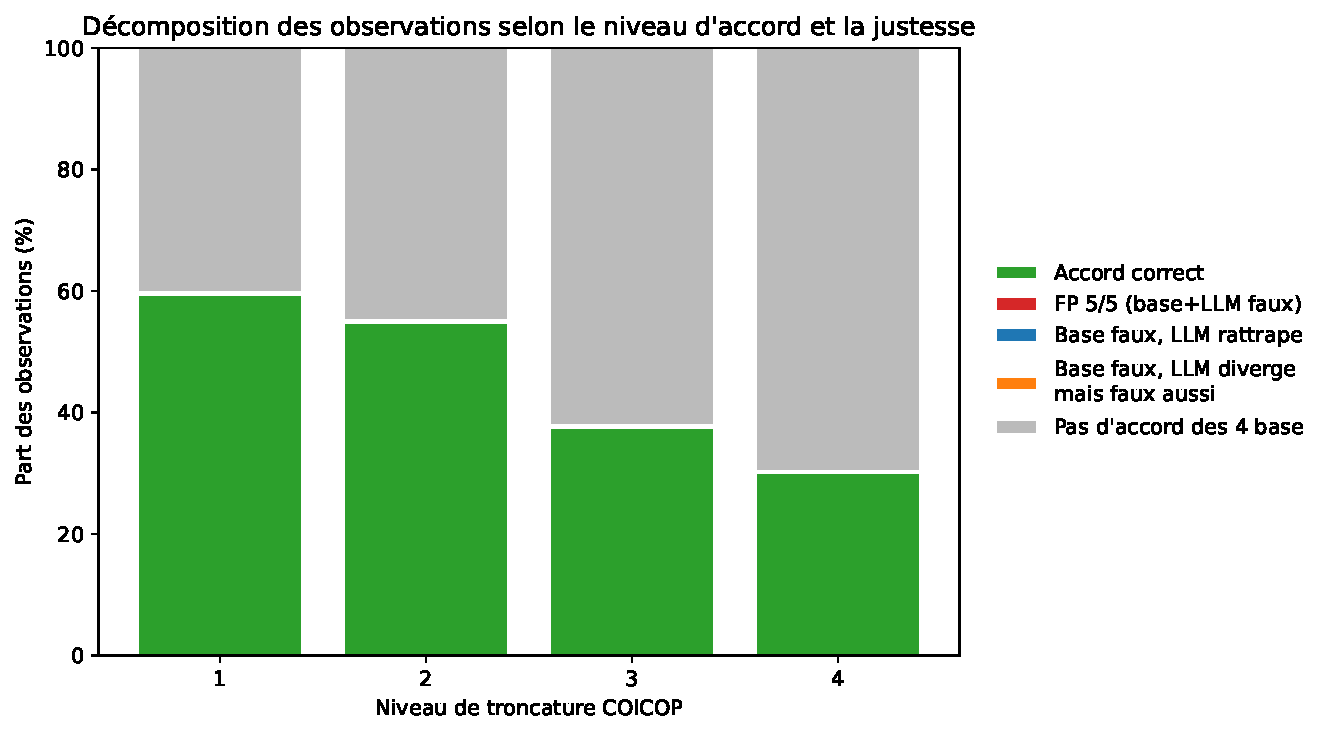
\includegraphics[keepaspectratio]{rapport_stage_files/figure-pdf/fig-recap-multi-niveaux-output-1.pdf}}

}

\caption{\label{fig-recap-multi-niveaux}Décomposition des observations
selon le niveau d'accord et la justesse, par niveau de troncature
COICOP}

\end{figure}%

Au niveau 4, les quatre classifieurs s'accordent sur 30.3\% des dépenses
; ce taux monte à 59.7\% si l'on se contente du niveau 1 (division), un
niveau de détail moins exigeant. Dans les deux cas, ce consensus est
presque toujours le bon : 99.2\% de justesse parmi les cas d'accord
unanime au niveau 4, et plus de 99\% à tous les niveaux (Figure 1).
L'accord unanime est donc un signal de confiance très fiable, quel que
soit le niveau de détail retenu.

\textbf{Trois classifieurs contre un dissident.} Lorsque trois
classifieurs sur quatre s'accordent contre un isolé (27.3\% des cas au
niveau 4), suivre la majorité reste globalement fiable : elle a raison
dans 91.5\% des cas, contre seulement 6.6\% pour le dissident --- même
si le risque d'erreur n'est ici plus négligeable.

\textbf{Un seul classifieur a raison.} À l'inverse, dans 8.7\% des cas,
un seul classifieur trouve le bon code contre les trois autres --- les
cas les plus difficiles, ceux où l'arbitrage du LLM-judge apporte le
plus de valeur ajoutée :

{

\begin{longtable}[]{@{}lll@{}}

\caption{\label{tbl-seul-correct}}

\tabularnewline

\toprule\noalign{}
& Effectif & Part des cas \\
Classifieur & & \\
\midrule\noalign{}
\endhead
\bottomrule\noalign{}
\endlastfoot
RAG-ANN & 464 & 91.9\% \\
TTC & 21 & 4.2\% \\
LLM-judge & 9 & 1.8\% \\
LCS & 8 & 1.6\% \\
RAG & 3 & 0.6\% \\

\end{longtable}

}

Ce classifieur « sauveur » est presque toujours \textbf{RAG-ANN}, loin
devant les trois autres : la recherche par similarité sur des libellés
déjà annotés par des gestionnaires s'avère, sur ces cas difficiles,
nettement plus précieuse que les notices officielles ou le classifieur
neuronal seuls.

\textbf{Autres signaux exploités.} Trois analyses complémentaires,
détaillées sur le site de suivi, confirment et affinent ce tableau : le
classement des trois meilleures propositions de TTC (et non son seul
rang 1) contient le bon code sensiblement plus souvent que le rang 1
seul, ce qui en fait une variable exploitable pour la suite ; les scores
de confiance natifs de chaque classifieur sont globalement bien calibrés
--- une confiance plus élevée correspond à une part de bonnes réponses
plus élevée, à des degrés variables selon le classifieur --- ce qui
justifie de les réutiliser comme variables explicatives en partie 3 ;
enfin, l'accuracy varie selon le mode de collecte (ticket de caisse
scanné contre saisie manuelle) et le montant de la dépense, sans
qu'aucun de ces deux facteurs ne domine largement les autres signaux
déjà identifiés.

\subsection{Un cadre reproductible pour rejouer l'étude sur un nouveau
run}\label{un-cadre-reproductible-pour-rejouer-luxe9tude-sur-un-nouveau-run}

Cette analyse n'a de valeur que si elle peut être rejouée à chaque
nouveau run de l'enquête, sans travail manuel. J'ai donc construit deux
outils distincts, complémentaires : un
\href{https://mathiskacer.github.io/codification_auto_coicop}{site de
suivi} au format Quarto, qui publie ces mêmes analyses (accord entre
classifieurs, calibration, modélisation) au fil des runs disponibles ;
et un rapport de statistiques descriptives autonome
(\texttt{rapport\_stat\_des/}), indépendant du site, paramétrable par le
chemin S3 d'un run via une simple variable d'environnement, et pensé
pour être branché directement dans le pipeline Argo existant plutôt que
généré à la main. Les résultats présentés dans ce rapport de stage
s'appuient sur ces mêmes outils, et resteront donc vérifiables et à jour
bien après sa rédaction.

\newpage

\section{Vote majoritaire et forêt aléatoire : une première alternative
au
LLM-judge}\label{vote-majoritaire-et-foruxeat-aluxe9atoire-une-premiuxe8re-alternative-au-llm-judge}

\emph{(à rédiger --- objectif de la partie : présenter la première
alternative opérationnelle au LLM-judge, construite directement à partir
des signaux identifiés dans la partie précédente.)}

\subsection{Le vote majoritaire comme règle de codification par
défaut}\label{le-vote-majoritaire-comme-ruxe8gle-de-codification-par-duxe9faut}

\emph{(à rédiger : la baseline --- vote majoritaire, arbitrage TTC ---
comme prolongement direct des constats d'accord entre classifieurs ;
aucune transformation de données supplémentaire n'est nécessaire ici.)}

\subsection{Une forêt aléatoire pour prédire la fiabilité du vote
majoritaire}\label{une-foruxeat-aluxe9atoire-pour-pruxe9dire-la-fiabilituxe9-du-vote-majoritaire}

\emph{(à rédiger : features et cible du modèle, formalisation en
prose/notation mathématique --- sans code ---, justification du choix
par rapport à d'autres modèles vus en 2A --- régression logistique,
arbre de décision unique. Méthodologie stricte résumée en une à deux
phrases, détail complet renvoyé en annexe.)}

\subsection{Ce que le modèle manque : analyse des erreurs non
détectées}\label{ce-que-le-moduxe8le-manque-analyse-des-erreurs-non-duxe9tectuxe9es}

\emph{(à rédiger : typologie des cas réannotés manuellement, limites du
modèle --- faux négatifs, sensibilité au seuil de décision --- ; moment
de discussion critique sur la portée du modèle.)}

\subsection{Arbitrer le volume envoyé au LLM selon le risque
accepté}\label{arbitrer-le-volume-envoyuxe9-au-llm-selon-le-risque-acceptuxe9}

\emph{(à rédiger : compromis précision/volume selon le seuil de
décision, préconisation chiffrée pour le SSP Lab.)}

\newpage

\section{SIRUS : transformer la confiance en règles métier
lisibles}\label{sirus-transformer-la-confiance-en-ruxe8gles-muxe9tier-lisibles}

\emph{(à rédiger --- objectif de la partie : présenter SIRUS comme
l'aboutissement lisible de la démarche --- formaliser la confiance en
règles métier auditables plutôt qu'en boîte noire.)}

\subsection{Pourquoi préférer des règles explicites à un modèle boîte
noire}\label{pourquoi-pruxe9fuxe9rer-des-ruxe8gles-explicites-uxe0-un-moduxe8le-bouxeete-noire}

\emph{(à rédiger : présentation de la méthode SIRUS --- principe,
formalisation, prérequis ---, développée dans le corps du texte car non
vue en cours ; justification par rapport à la forêt aléatoire classique
de la partie 3. Référence bibliographique : papier SIRUS.)}

\subsection{Reformuler les données en une décision par candidat plutôt
que par
produit}\label{reformuler-les-donnuxe9es-en-une-duxe9cision-par-candidat-plutuxf4t-que-par-produit}

\emph{(à rédiger : construction de la table longue candidat-level,
sentinelles utilisées ; méthodologie du split train/test par produit,
propre à cette structure de données.)}

\subsection{Les règles retenues et leur pouvoir de
discrimination}\label{les-ruxe8gles-retenues-et-leur-pouvoir-de-discrimination}

\emph{(à rédiger : règles SIRUS effectivement retenues, calibration de
la confiance, features additionnelles testées sans gain --- résultat
négatif interprété ---, réglage des hyperparamètres.)}

\subsection{Une performance qui plafonne : généralisation à de nouveaux
runs}\label{une-performance-qui-plafonne-guxe9nuxe9ralisation-uxe0-de-nouveaux-runs}

\emph{(à rédiger : accuracy comparée sur plusieurs runs --- cf.~la
comparaison McNemar déjà calculée sur le site ---, écart RAG-ANN
documenté comme point ouvert et non tranché ; moment de discussion
critique sur la portée de l'étude.)}

\newpage

\section{Conclusion}\label{conclusion}

\emph{(à rédiger en dernier, une fois le plan et le message central
stabilisés : bilan comparatif explicitement relié à la thèse défendue ;
discussion assumée d'un projet en cours, non figé --- troncature et
écart RAG-ANN comme limites assumées, pas comme des échecs --- ;
perspectives et préconisations chiffrées pour le SSP Lab.)}

\newpage
\bibliographie{bibliographie}{plain}

\emph{(à compléter : sources effectivement citées dans le corps du texte
uniquement --- SIRUS (Bénard, Biau, Da Veiga, Scornet), Hastie,
Tibshirani \& Friedman,} The Elements of Statistical Learning \emph{(si
citée pour la formalisation RF/CART), documentation COICOP/Eurostat,
documentation du pipeline existant
(\texttt{inseefrlab/codif-coicop-bdf}).)}

\newpage
\annexes

\section{Méthodologie détaillée de la forêt
aléatoire}\label{annexe-pipeline}

\emph{(à compléter : détail du pipeline de codification existant ---
prétraitement, règles regex, fonctionnement des 4 classifieurs (LCS,
RAG-notices, RAG-annotations, TTC) --- renvoyé ici depuis la partie 1.3
pour ne pas alourdir le corps ; puis méthodologie complète de la forêt
aléatoire --- encodage, imputation, split, validation croisée, recherche
d'hyperparamètres.)}

\section{Table complète de réannotation
manuelle}\label{table-compluxe8te-de-ruxe9annotation-manuelle}

\emph{(à compléter : les cas réannotés à la main, référencés en 3.3.)}

\section{Détail des hyperparamètres
SIRUS}\label{duxe9tail-des-hyperparamuxe8tres-sirus}

\emph{(à compléter : résultats de la recherche/validation croisée
SIRUS.)}

\section{Règles SIRUS extraites}\label{ruxe8gles-sirus-extraites}

\emph{(à compléter : liste complète des règles retenues, sortie
\texttt{sirus.print}.)}

\section{Bilan personnel}\label{bilan-personnel}

\emph{(à compléter --- 1 à 2 pages : compétences acquises, intégration
dans l'équipe et l'environnement professionnel. Ne doit apparaître
qu'ici, pas dans le corps ni la conclusion.)}

\section{Liens utiles}\label{liens-utiles}

\emph{(à compléter : lien du site de suivi, lien du dépôt.)}




\end{document}
